
\chapter{Motivation}
\section{Inspiration}
Inspired by the movie \textit{2001: A Space Odyssey} produced and directed by Stanley Kubrick, an adaption has been created by using POV-Ray. The adaption contains selected scenes of 5 minute clip on youtube.  With the exception of few scenes the cuts and scenes as well as the soundtrack are geared to the original video \cite{EbClectic}.

\chapter{Models}
The whole short animation is created in POV-Ray. Everything but the starships (section \ref{imported_models}) has been created from scratch without using any external tools.
\section{Imported Models} \label{imported_models}

We found the models of the Orion III Spaceplane (figure \ref{orion}) and Space Station V (figure \ref{station}) by B.J. West with textures by Michael Powell in the \textit{2001: A Space Odyssey 3D Modelling Archiv} \cite{Archive}.
Since both models were not available in a format directly usable with POV-Ray but \textit{3ds Max} (former called \textit{3D Studio Max}), we had to convert them from Autodesks proprietary format (.max) to the open Wavefront .obj format, which we then converted to POV-Ray code using PoseRay \cite{PoseRay}.
\begin{figure} [ht]
	\subfigure[Orion]{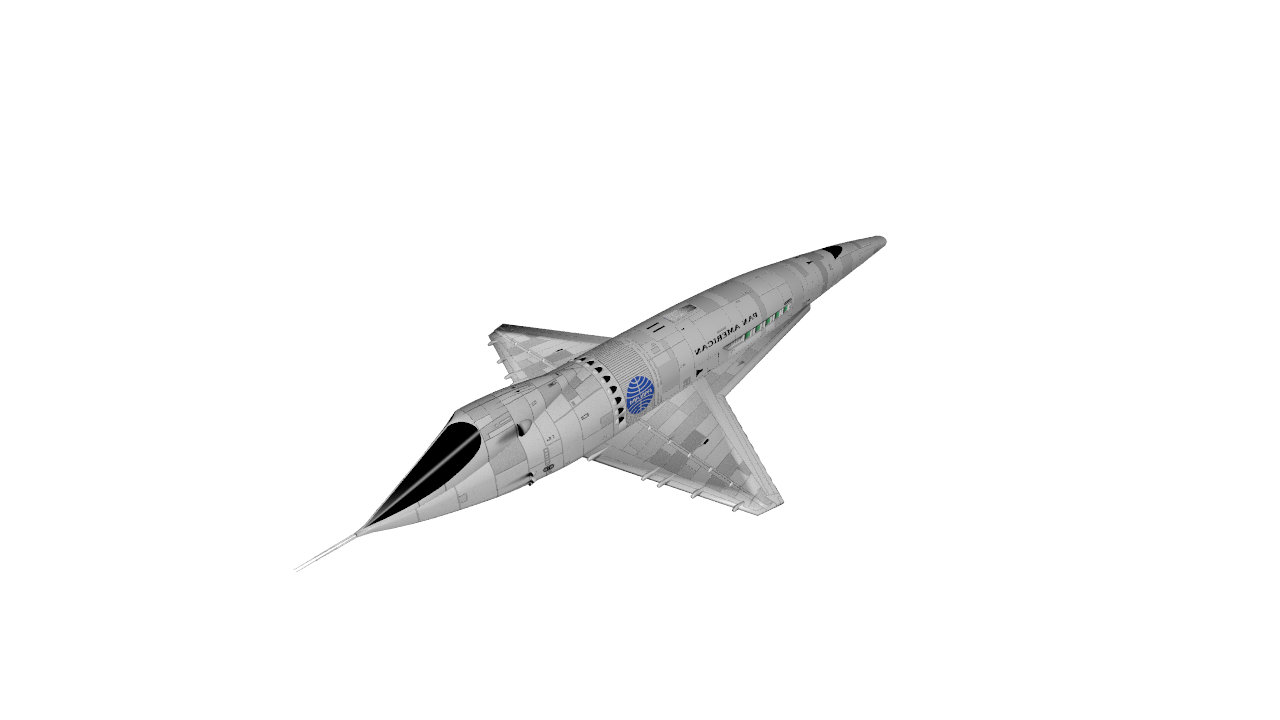
\includegraphics[width=0.55\textwidth]{images/orion.jpg} \label{orion} } 
	\subfigure[Space Station V]{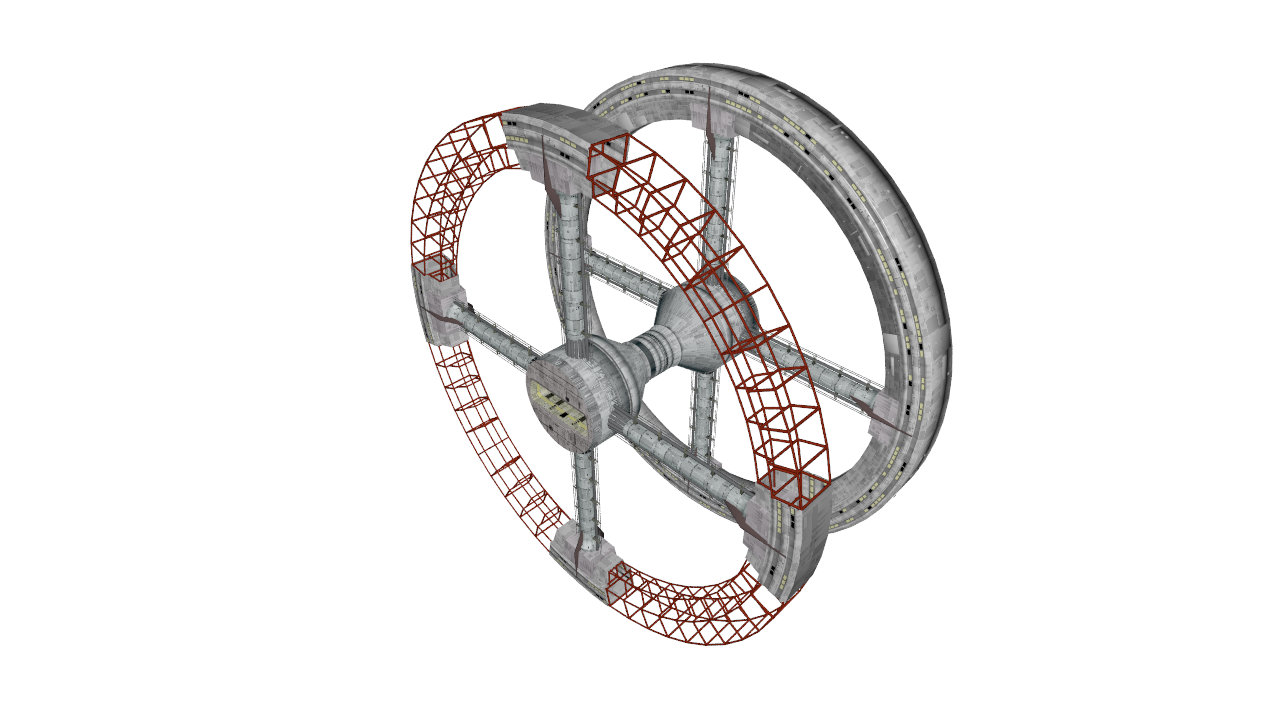
\includegraphics[width=0.6\textwidth]{images/station.jpg}	\label{station}} 
	\caption{Imported Models: Left \textit{Orion}, Right \textit{Station V}} 
\end{figure} 

\newpage
\section{Remarkable Models}

\subsection{Human} \label{human_model}

The human is likely the most complex of the models we created, due to the hierarchy of connected parts.
It consists of 13 individually poseable parts (three per limb and one for the head), that are connected via the torso.
Each part is connected to either their direct parent part (i.e. the hand is connected to the underarm, which is connected to the upper arm) or the torso.
The model can be posed (and animated) by assinging the rotation vectors to certain variables (see code below) before calling the macro that inserts the model.
It also has a special mode that replaces the used textures with transparent ones and visualizes the alignment of the x, y and z axis at the point of each joint (see figure \ref{fig_human}).

\begin{lstlisting}
object {
    #local DEBUG_ALL_JOINTS = false;
    #local LEFT_ARM_ROT = <0, 90, 0>;
    #local LEFT_LOWER_ARM_ROT = <45, 0, 0>;
    ...

    Human()
}
\end{lstlisting}

\begin{figure}[ht]
	\centering
	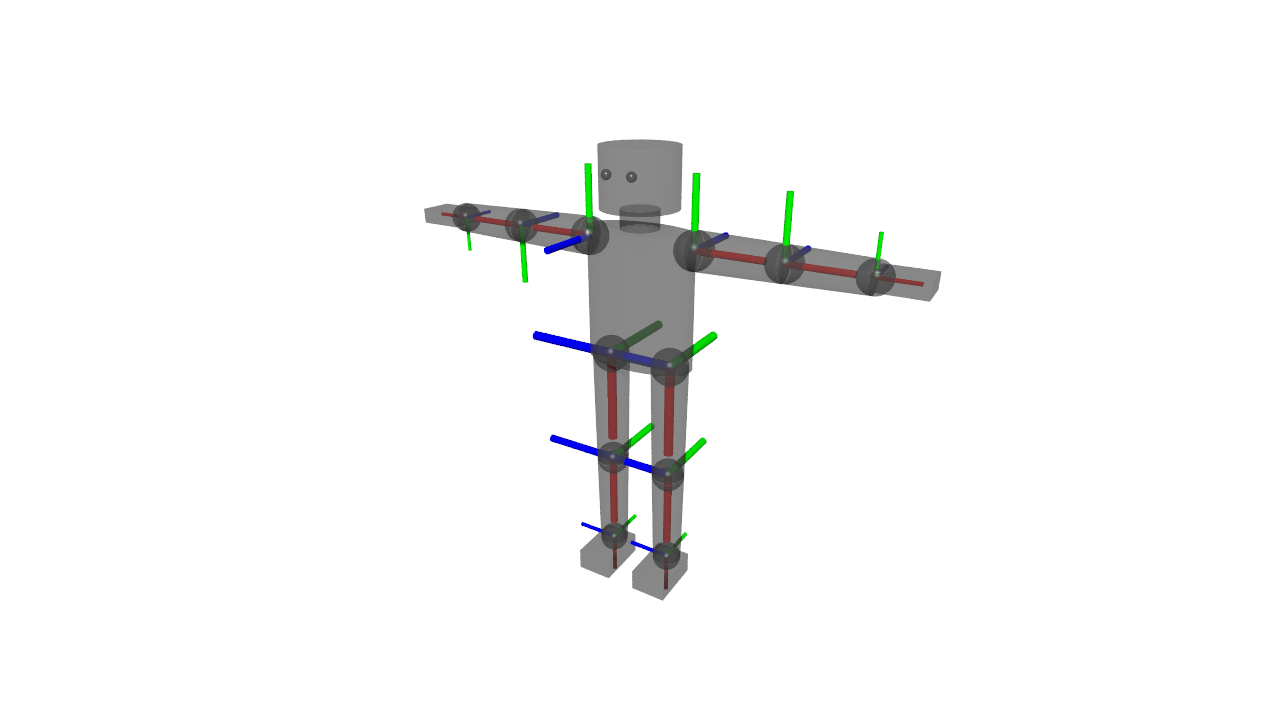
\includegraphics[width=0.85\textwidth]{images/human.png}
	\caption{Simple humanoid model in the default pose (with debug mode being active)}
	\label{fig_human}
\end{figure}

\newpage
\subsection{Cabin}

The model of the cabin (figure \ref{cabin}) is built after the original (figure \ref{cabin_original}) using only boxes that are rotated and translated. The seats are duplicated using two for loops.

\begin{figure}[ht]
	\centering
	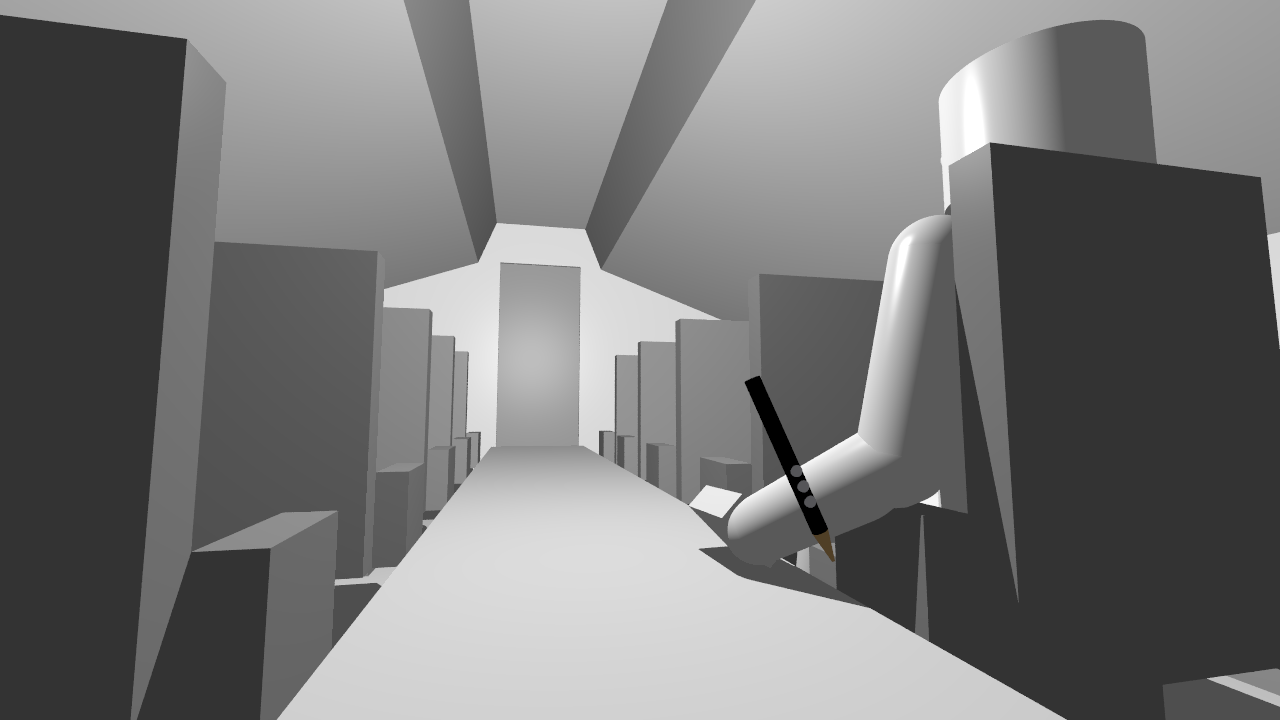
\includegraphics[width=0.85\textwidth]{images/cabin.png}
	\caption{Cockpit of Starship \textit{Orion} built in POV-Ray.}
	\label{cabin}
\end{figure}

\begin{figure}[ht]
	\centering
	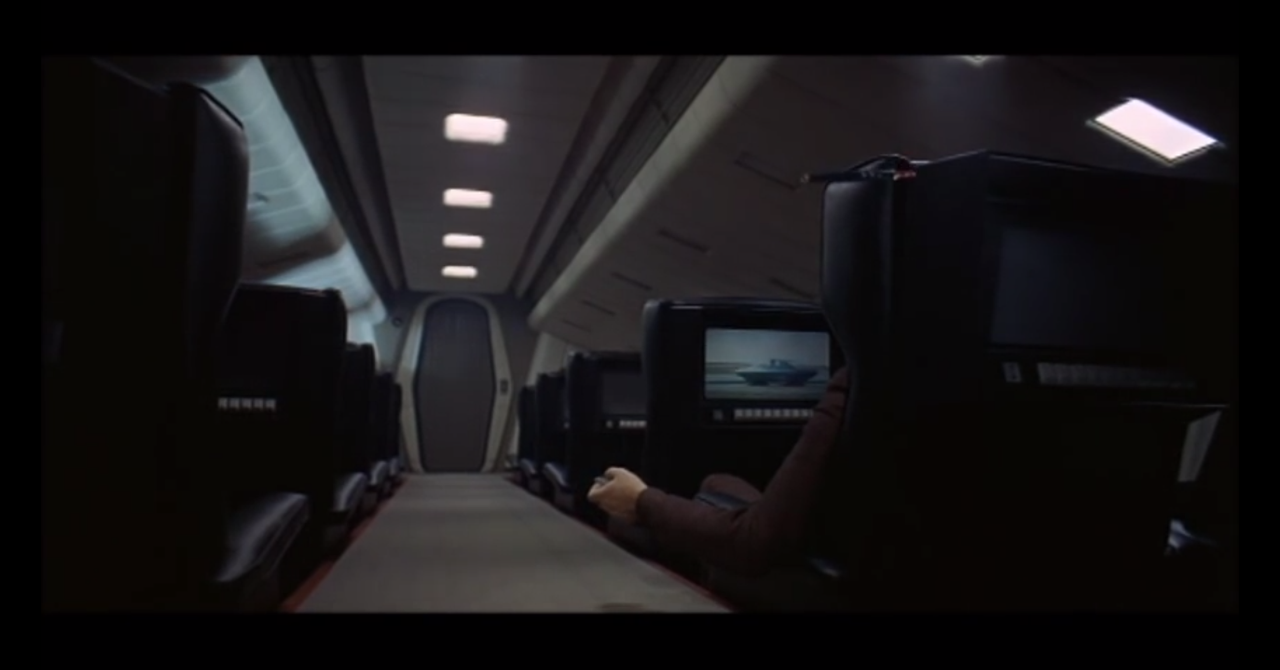
\includegraphics[width=0.85\textwidth]{images/cabin_original.png}
	\caption{Cabin of Starship \textit{Orion} taken from \textit{2001: A Space Odyssey}}
	\label{cabin_original}
\end{figure}

\newpage
\subsection{Cockpit} \label{cockpit_model}
Inspired by the cockpit (figure \ref{cockpit_original}) shown in the movie, the cockpit in the adaption  is built completely from scratch using POV-Ray (figure \ref{cockpit_povray}). The starship \textit{Station} on this scene belongs to the imported models (section \ref{imported_models}).
The pilots are transformed models of the human (subsection \ref{human_model}).

\begin{figure}[ht]
	\centering
	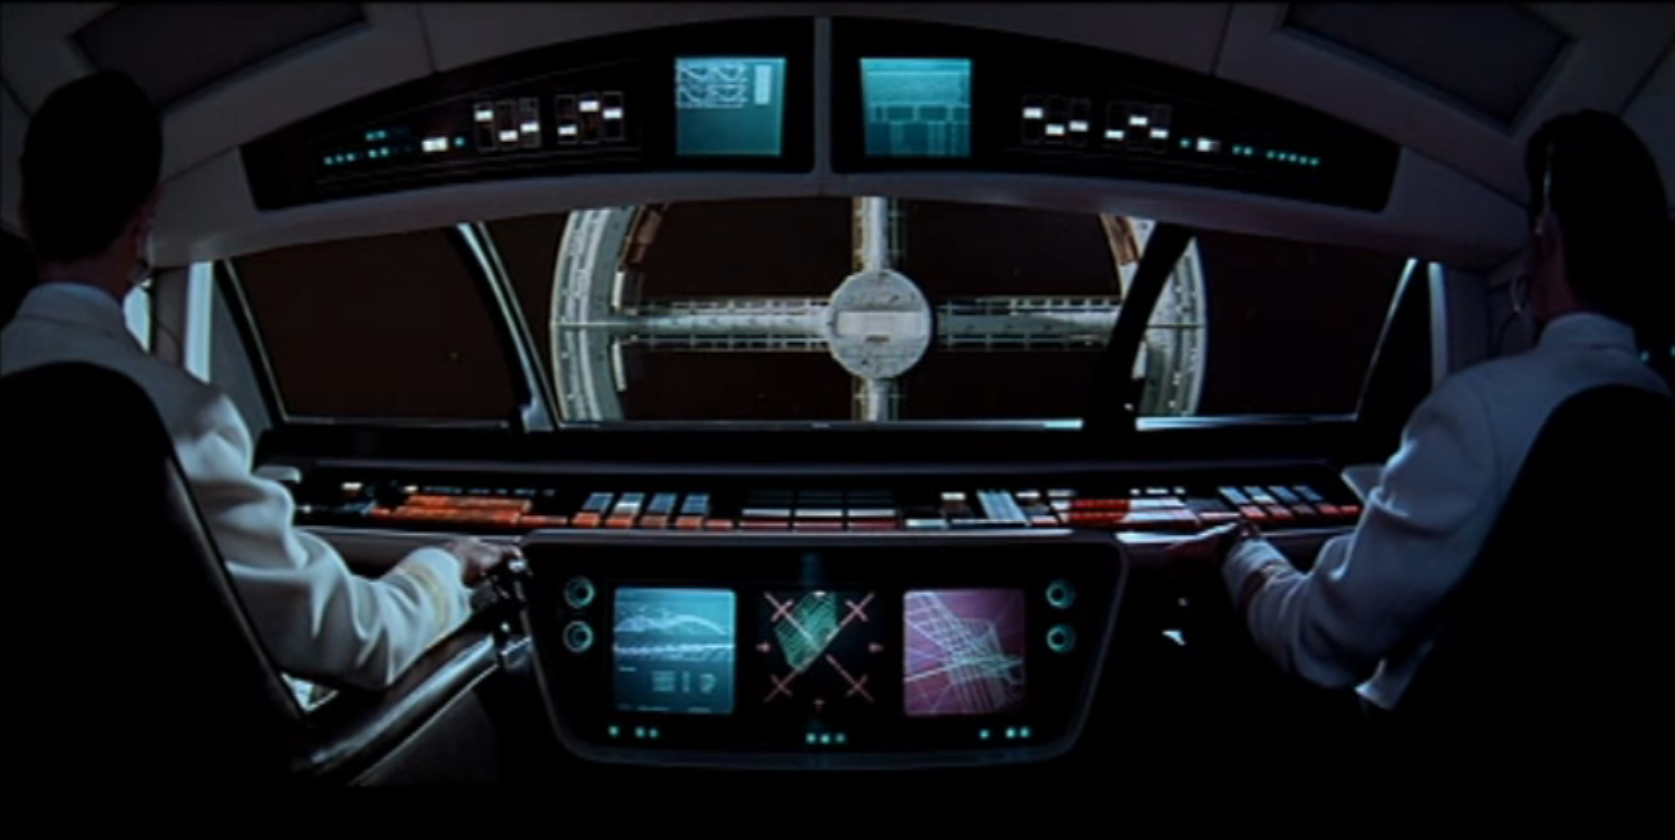
\includegraphics[width=0.85\textwidth]{images/original_cockpit.png}
	\caption{Cockpit of Starship \textit{Orion} taken from \textit{2001: A Space Odyssey}}
	\label{cockpit_original}
\end{figure}

\begin{figure}[ht]
	\centering
	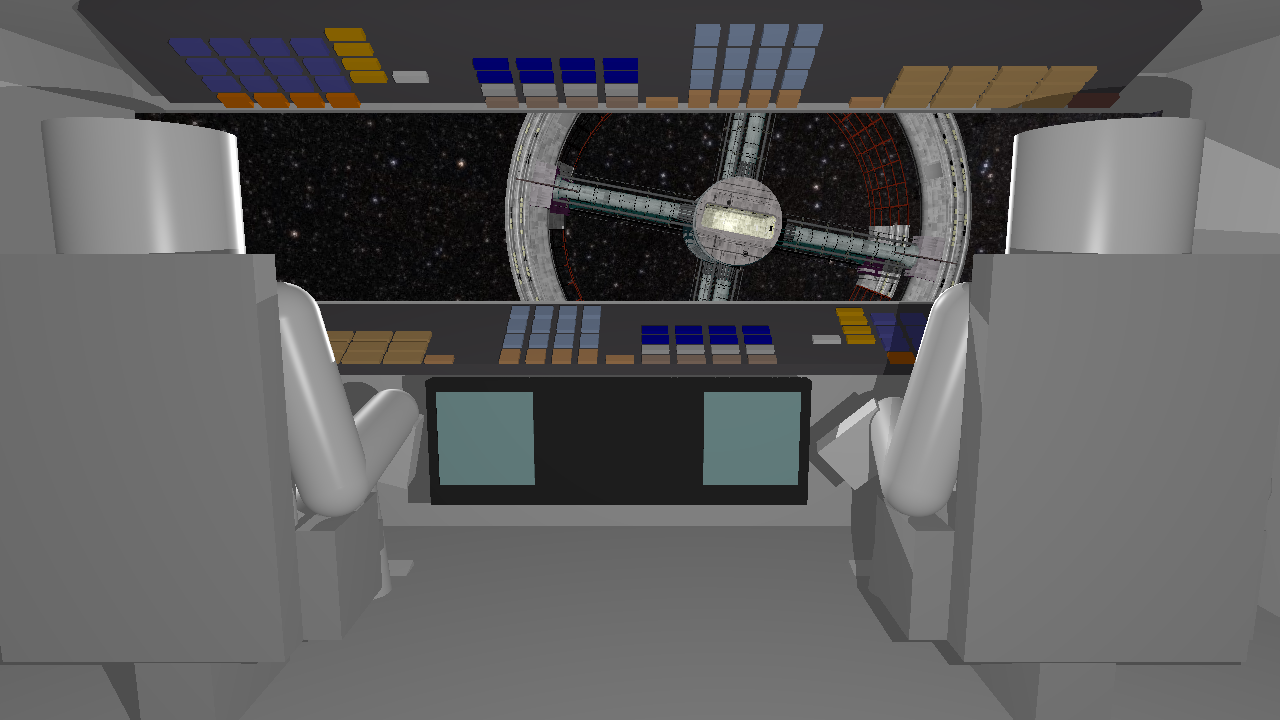
\includegraphics[width=0.85\textwidth]{images/scene19587.png}
	\caption{Cockpit of Starship \textit{Orion} built in POV-Ray.}
	\label{cockpit_povray}
\end{figure}

The associated POV-Ray script can be found on GitHub \cite{Quving}.

\newpage
\subsection{Planet}
As well as the cockpit (\ref{cockpit_model}) the planet shown in figure \ref{planet_original} has been recreated in POV-Ray (figure \ref{planet_povray}).
\begin{figure}[ht]
	\centering
	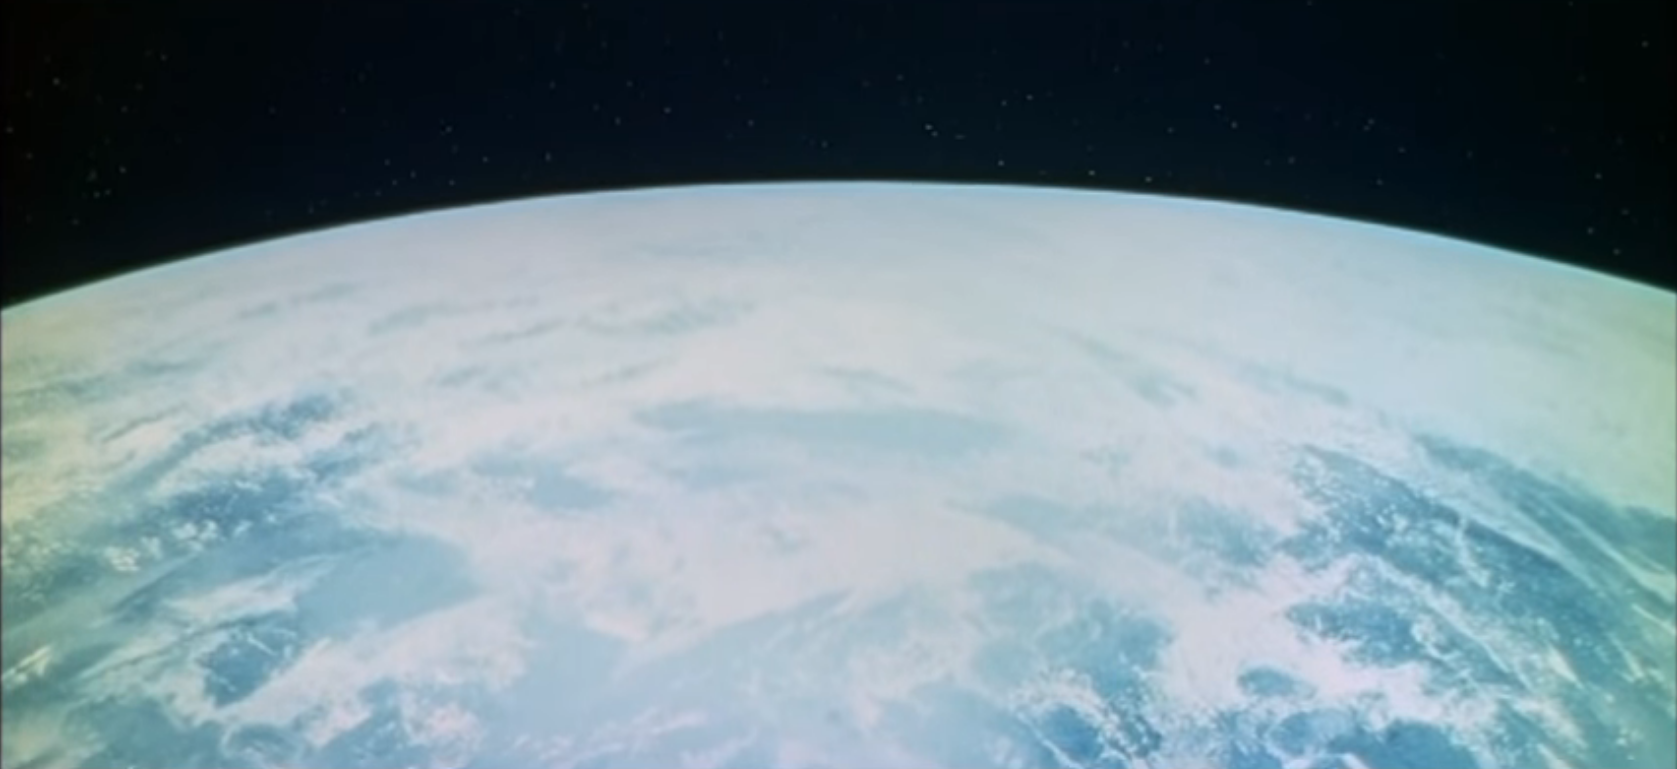
\includegraphics[width=0.85\textwidth]{images/original_planet.png}
	\caption{A picture of a planet taken from \textit{2001: A Space Odyssey}.}
	\label{planet_original}
\end{figure}

\begin{figure}[ht]
	\centering
	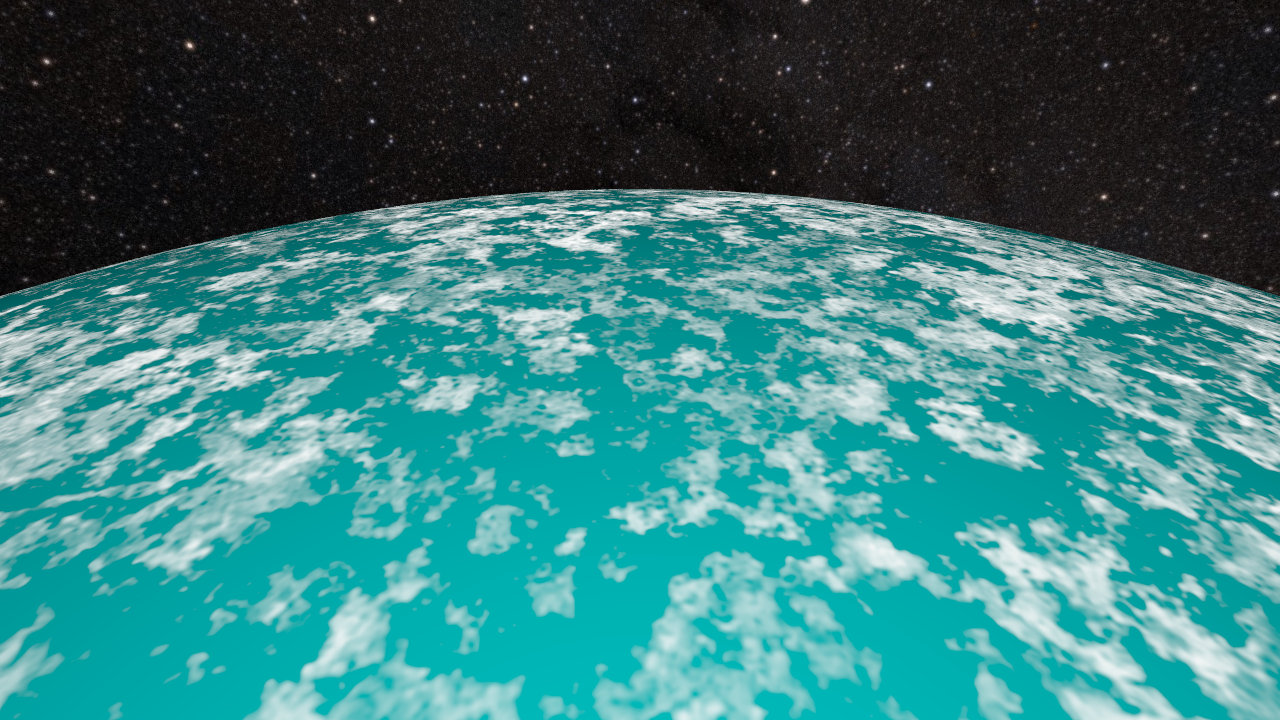
\includegraphics[width=0.85\textwidth]{images/scene04_05.jpg}
	\caption{This figure shows the result of a recreation of the above shown planet (\ref{planet_original}).}
	\label{planet_povray}
\end{figure}

The associated POV-Ray script can be found on GitHub \cite{Quving} and in the section \ref{povray_snippets}.

\newpage
\section{POV-Ray Snippets} \label{povray_snippets}

\subsection{Planet}

\begin{lstlisting}
#declare PLANET = sphere {
	0, 5000
	rotate <clock*15, 0, 0>
	pigment { color rgb <0,0.75,0.75> }
	finish { ambient 0.00 diffuse 1}
	texture{
		pigment{
			bozo turbulence 0.075
			octaves 6  omega 0.7 lambda 2
			color_map {
				[0.0  color rgb <0.95, 0.95, 0.95> ]
				[0.05  color rgb <1, 1, 1>*1.25 ]
				[0.15 color rgb <0.85, 0.85, 0.85> ]
				[0.55 color rgbt <1, 1, 1, 1>*1 ]
				[1.0 color rgbt <1, 1, 1, 1>*1 ]
			}
		}
		finish { ambient 0 diffuse 1}
	}
}
\end{lstlisting}

\chapter{Production}

\section{Rendering} \label{rendering}
Once the frames are generated by POV-Ray, they were put together to a mp4 video by using \textit{ffmpeg}.
The following command renders frames with the format \texttt{sceneXX\_YYY.png} with 60 frame per second.

\begin{lstlisting}
$ ffmpeg \
  -r 60 \
  -start_number 1 \
  -i scenex_%03d.png \
  -c:v libx264 \
	-strict experimental \
	-tune fastdecode \
	-pix_fmt yuv420p\
	-b:v 1500k \
	out.mp4

\end{lstlisting}

\section{Post-Production}

Each scene is represented by a video obtained as above described (section \ref{rendering}). The final video and the soundtrack are cut by using \textit{Vegas Pro 14.0} \cite{VegasPro} on Windows.
